\section{Hall Thruster Types}
\subsection{Annular Hall Thrusters}
\ac{AHT}s are the most common type of \ac{HET} in use today. They feature an axisymmetrical annular discharge channel where tne propellant is ionized and accelerated. The magnetic field is generated by coaxial coil windings wrapped in and around the discharge channel or by permanent magnets. It consists on a high voltage metallic anode located upstream in the channel, and a cathode that is often located outside the channel.

In-space thruster tests with this geometry have demonstrated thrusts up to 280mN. They have exhibited power levels of up to 4.5kW, and specific impulses up to 2000s. \cite{bpt-4000} \cite{spt-140} \\

\begin{figure}[H]
    \centering
    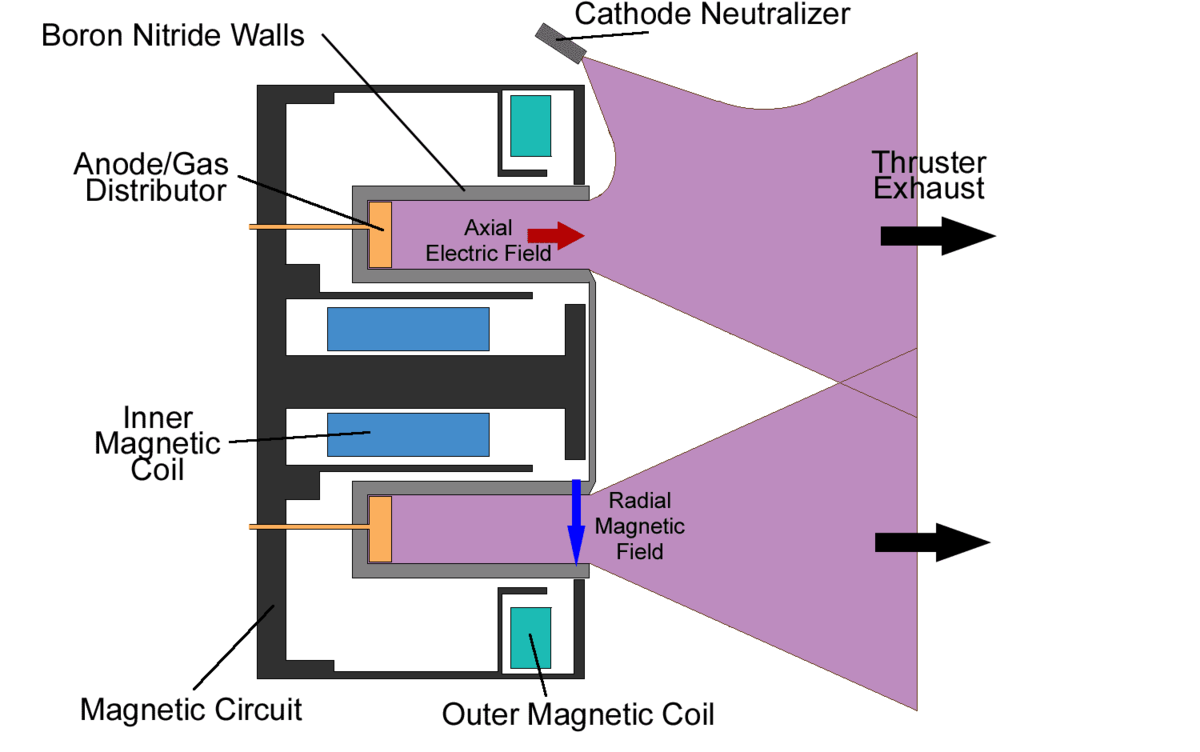
\includegraphics[width=0.7\textwidth]{images/Concepts/Annular HET.png}
    \captionsetup{justification=centering}
    \caption{Annular \ac{HET}}
    \label{fig:annular_HET}
\end{figure}


\subsection{Cylindrical Hall Thrusters}

One of the largest drawbacks when downscaling \ac{AHT}s is the increase in surface area to volume ratio, which leads to higher wall losses and lower efficiency. The plasma tends to interact with the thruster channel walls, which results in heating and erosion of the thruster parts \cite{cht-plasma-wall-interactions}. To combat this, \ac{CHT}s, proposed at the Princeton Plasma Physics Laboratory were developed. As seen in figure \ref{fig:cylindrical_HET}, the ratio of the channel surface area to volume is reduced, limiting electron transport and ion losses \cite{pppl-cht}. These thrusters have also seen unusually high propellant ionization efficiencies, hence being able to operate at much lower discharge voltages and propellant flow rates \cite{cht-vs-aht}.

\begin{figure}[H]
    \centering
    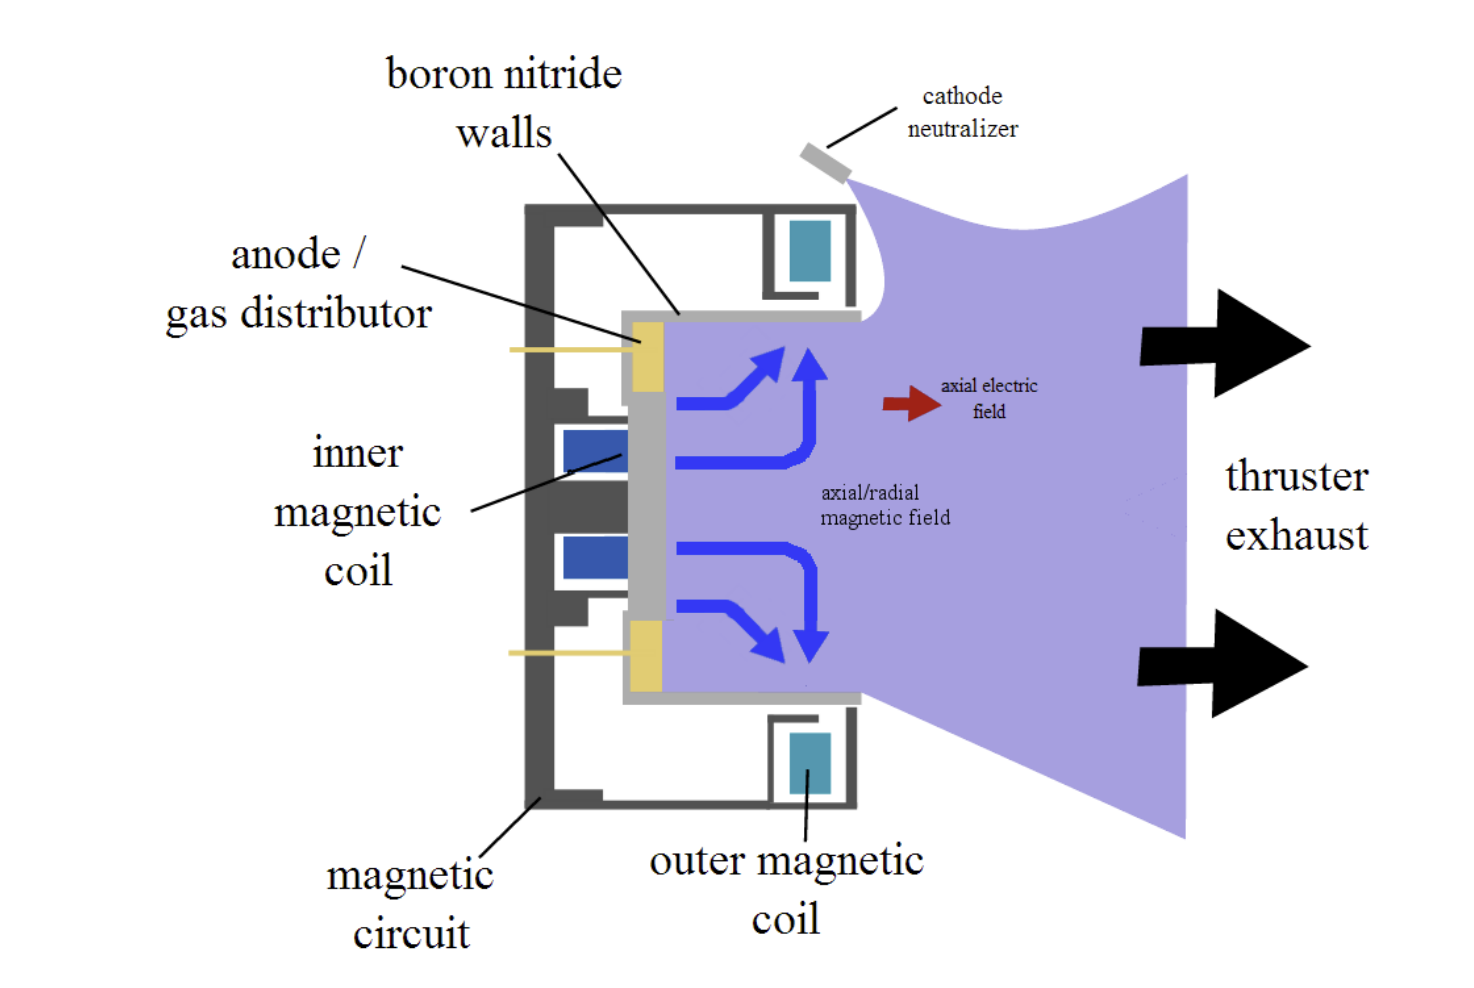
\includegraphics[width=0.7\textwidth]{images/Concepts/CHT.png}
    \captionsetup{justification=centering}
    \caption{Cylindrical \ac{HET} \cite{pigeon2017development}}
    \label{fig:cylindrical_HET}
\end{figure}